% !TeX spellcheck = en_US
\documentclass[letterpaper,12pt,twoside]{report}
\usepackage{fancyhdr}
\usepackage{fullpage}
\usepackage{tikz}
\usepackage{amsmath}
\usepackage{textcomp}
\usepackage{longtable}
%\usepackage{TwoColumnProof}

\begin{document}
	\pagestyle{fancy}
	\fancyhf{}
	\fancyhead[L]{Day 6}
	\fancyhead[R]{\textit{The Calendar Project}}
	\fancyfoot[L]{Citations Involved: none}
	
	% Problem
	\paragraph{Problem}
	\begin{quote}
	\textsf{An equilateral triangle is inscribed in a circle of radius 6 in. A second equilateral triangle is circumscribed about the circle. If the sides of the triangles are parallel, what is the shortest distance from a point on one triangle to a point on the other?}
	\end{quote}
	
	% Graphics
	\begin{center}
		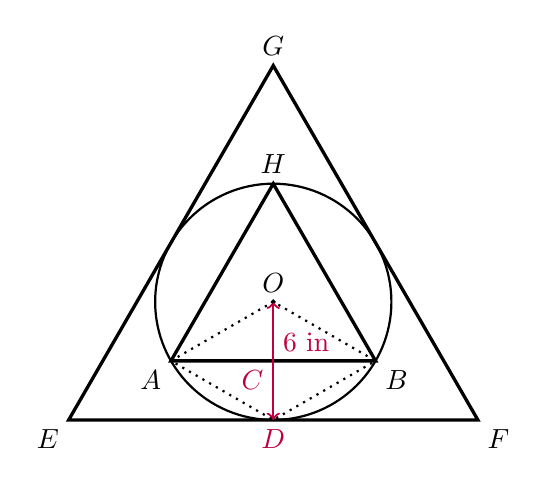
\begin{tikzpicture}[scale=0.25]
		\draw[thick] (0,0) circle [radius=6];
		\draw[very thick] (0,6) -- (-5.19615,-3) -- (5.19615,-3) -- cycle;
		\draw[very thick] (0,12) -- (-10.3923,-6) -- (10.3923,-6) -- cycle;
		
		\draw[fill=black] (0,0) circle [radius=0.1];
		\node[above] at (0,0) {$O$};
		
		\draw[<->][thick][purple] (0,0) -- (0,-6);
		\node[below][purple] at (0,-6) {$D$};
		\node[above right][purple] at (0,-3) {$6$ in};
		\node[below left][purple] at (0,-3) {$C$};
		
		\draw[dotted][thick] (-5.19615,-3) -- (0,0) -- (5.19615,-3) -- (0,-6) -- cycle;
		\node[below left] at (-5.19615,-3) {$A$};
		\node[below right] at (5.19615,-3) {$B$};
		\node[below left] at (-10.3923,-6) {$E$};
		\node[below right] at (10.3923,-6) {$F$};
		\node[above] at (0,12) {$G$};
		\node[above] at (0,6) {$H$};
		\end{tikzpicture}
	\end{center}
	
	% Reasoning
	\paragraph{Reasoning}
	\begin{quotation}
	
	The shortest distance between two parallel lines is the length of the perpendicular segment that connects them. Given that $\overline{AB} \parallel \overline{EF}$, draw $\overline{OD}$ as a radius of circle $O$ such that $\overline{OD}\bot\overline{AB}$; as such, $\overline{OD}\bot\overline{EF}$ by the Perpendicular Transversal Theorem (2). Since $\overline{OD}$ is a radius perpendicular to chord $AB$, it bisects $\overline{AB}$ (14); therefore $\overline{OD}$ is a perpendicular bisector of $\overline{AB}$. Let the point of intersection between $\overline{AB}$ and $\overline{OD}$ be $C$; since $\overline{OD}$ bisects $\overline{AB}$, $C$ is equidistant from $A$ and $B$; therefore $AC=CB$. Since $\overline{OD}\bot\overline{AB}$, $\angle ACO$, $\angle BCO$, $\angle ACD$, and $\angle BCD$ are right angles and have measures that are equal to 90\textdegree.
	
	Since an equilateral triangle is also equiangular (9), it is a regular polygon by definition (11). Since the central angle of a regular $n$-gon is $\frac{360\text{\textdegree}}{n}$ (12), and since a triangle has 3 sides, the central angle of an equilateral triangle is $\frac{360\text{\textdegree}}{3}=120$\textdegree; since $\angle AOB$ is a central angle of a regular polygon by definition (12), its measure is 120\textdegree. Since $\overline{OA}$, $\overline{OD}$, and $\overline{OB}$ are radii of circle $O$, they are congruent and are given to be 6 inches long. In $\triangle OAB$, with $\overline{OA}\cong\overline{OB}$, $\angle OAB\cong\angle OBA$ and therefore $\text{m}\angle OAB=\text{m}\angle OBA$ by the Isosceles Triangle Theorem (8). By the Triangle Sum Theorem (5), $\text{m}\angle AOB+\text{m}\angle OAB+\text{m}\angle OBA=180$\textdegree; after substitution, $120+\text{m}\angle OAB+\text{m}\angle OBA=180 \Rightarrow \text{m}\angle OAB+\text{m}\angle OBA=180-120=60$; thus $\text{m}\angle OAB=\text{m}\angle OBA=\frac{60}{2}=30$. By the Triangle Sum Theorem (5), $\text{m}\angle OAC+\text{m}\angle ACO+\text{m}\angle COA=180$\textdegree \space and $\text{m}\angle OBC+\text{m}\angle BCO+\text{m}\angle COB=180$\textdegree. After respective substitution, $30+90+\text{m}\angle COA=180$ and $30+90+\text{m}\angle COB=180$; thus $\text{m}\angle COA=180-30-90=60$ and $\text{m}\angle COB=180-30-90=60$. By the 30\textdegree-60\textdegree-90\textdegree \space Triangle Theorem (10), $AO=2CO$ and $BO=2CO \Rightarrow CO=\frac{AO}{2}$; with $AO=6$, $CO=\frac{6}{2}=3$ by substitution. By the SAP, $CO+CD=OD$; with $OD=6$ and $CO=3$, $3+CD=6 \Rightarrow CD=6-3=\boxed{3 \text{  in}}$. Since $\overline{CD}$ is a perpendicular segment that connects parallel sides of the two triangles, its length is the solution to this problem.
	\end{quotation}

	\paragraph{Alternative Solution}
	\begin{quotation}
		Draw circle $O$ with radius 6 in. Circumscribe circle $O$ with $\triangle EGF$ such that $\triangle EGF$ is an equilateral triangle. Connect the points of tangency between the sides of $\triangle EGF$ and circle $O$ to construct $\triangle ABH$.
	\end{quotation}
		\begin{center}
		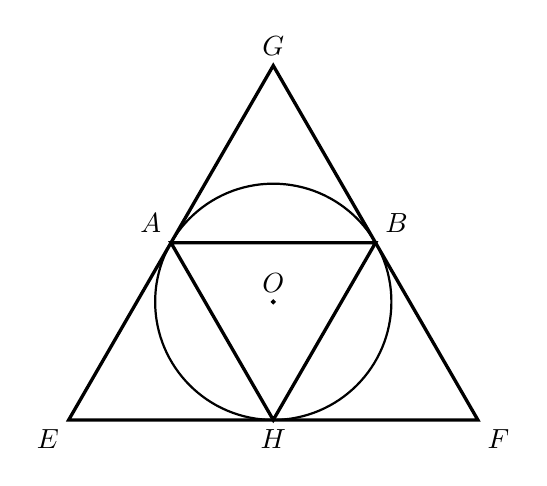
\begin{tikzpicture}[scale=0.25]
		\draw[thick] (0,0) circle [radius=6];
		\draw[very thick] (-5.19615,3) -- (5.19615,3) -- (0,-6) -- cycle;
		\draw[very thick] (0,12) -- (-10.3923,-6) -- (10.3923,-6) -- cycle;
		
		\draw[fill=black] (0,0) circle [radius=0.1];
		\node[above] at (0,0) {$O$};
		
		\node[above left] at (-5.19615,3) {$A$};
		\node[above right] at (5.19615,3) {$B$};
		\node[below left] at (-10.3923,-6) {$E$};
		\node[below right] at (10.3923,-6) {$F$};
		\node[above] at (0,12) {$G$};
		\node[below] at (0,-6) {$H$};
		\end{tikzpicture}
		\end{center}
	
	\begin{quotation}
		Because the inscribed triangle and the circumscribed triangle touch each other at the vertices of the inscribed triangle, the shortest distance between them is $\boxed{0}$. The proof that this follows the constraints in the problem is below.
	\end{quotation}
	
	\begin{tabular}{l}
		\textbf{Given: } $\triangle GEF$ circumscribes circle $O$; $\triangle GEF$ is an equilateral triangle \\
		\textbf{Prove: } $\overline{AB}\parallel\overline{EF}$; $\overline{AH}\parallel\overline{GF}$; $\overline{BH}\parallel\overline{GE}; \triangle ABH$ is an equilateral triangle
		\end{tabular}
	
		\newcounter{proofstmt}
		\newcommand{\StatementReason}[2]{
			\refstepcounter{proofstmt}
			\theproofstmt. & #1 & \theproofstmt. & #2 \\
		}
	\setcounter{proofstmt}{0}
	\renewcommand{\arraystretch}{1.15}
		\begin{longtable}{|l p{0.41\linewidth} l p{0.41\linewidth}|}
			\hline
			& \textbf{Statement} & & \textbf{Reason} \\
			\hline
			\StatementReason{$\triangle GEF$ is an equilateral triangle}{Given}
			\StatementReason{$\triangle GEF$ is an equiangular triangle}{Equilateral $\triangle$s are equiangular (9)}
			\StatementReason{$\text{m}\angle GEF=\text{m}\angle EFG=\text{m}\angle FGE=60$\textdegree}{The measure of each $\angle$ of an equiangular $\triangle$ is 60\textdegree \space(3)}
			% TODO \StatementReason{$\overline{EG},\overline{GF},\text{and }\overline{FE}$ are tangent to circle $O$.}
			\StatementReason{$\overline{AE}\cong\overline{HE}, \overline{BF}\cong\overline{HF}, \overline{AG}\cong\overline{BG}$}{2 segs. tangent to same circle from same ext. pt. $\rightarrow$ segs $\cong$ (7)}
			\StatementReason{$AE=HE, BF=HF, AG=BG$}{Definition of segment $\cong$}
			\StatementReason{$\angle GEF\cong\angle EFG\cong\angle FGE$}{Definition of equiangular $\triangle$s (3)}
			\StatementReason{$\overline{EG}\cong\overline{GF}\cong\overline{FE}$}{Definition of equilateral $\triangle$s (4)}
			\StatementReason{$EG=GF=FE$}{Definition of segment $\cong$}
			\StatementReason{$AE+AG=EG$, \par $BG+BF=GF$, \par $HF+HE=FE$}{SAP}
			\StatementReason{$AE+AG=BG+BF=HF+HE$}{Substitution}
			\StatementReason{$AE+AG=AG+BF=BF+AE$}{Substitution}
			\StatementReason{$AE=BF, AG=AE$}{Subtraction Property of =}
			\StatementReason{$AE=BF=HE=HF=AG=BG$}{Transitive Property}
			\StatementReason{$\overline{AE}\cong\overline{BF}\cong\overline{HE}\cong\overline{HF}\cong\overline{AG}\cong\overline{BG}$}{Definition of segment $\cong$}
			\StatementReason{$\angle AEH\cong\angle BFH\cong\angle BGA$}{Reflexive Property (Step 6)}
			\StatementReason{$\triangle AEH\cong\triangle BFH\cong\triangle BGA$}{SAS (7)}
			\StatementReason{$\overline{AH}\cong\overline{BH}\cong\overline{BA}$}{CPCTC}
			\StatementReason{$\triangle ABH$ is an equilateral $\triangle$}{Definition of equilateral $\triangle$s}
			\StatementReason{$\angle BAG\cong\angle HEA$,\par $\angle EHA\cong\angle HFB$,\par $\angle FBH\cong\angle BGA$}{CPCTC}
			\StatementReason{$\overline{AB}\parallel\overline{EF}$, $\overline{AH}\parallel\overline{GF}$, $\overline{BH}\parallel\overline{GE}$}{Converse of the Corresponding $\angle$s Postulate (1)}
			\hline
		\end{longtable}
	
	
	\paragraph{External References}
	\begin{enumerate}
		\item Textbook Ch. 3, Pg. 162: Converse of the Corresponding $\angle$s Postulate
		\item Textbook Ch. 3, Pg. 173: Perpendicular Transversal Theorem
		\item Textbook Ch. 4, Pg. 216: Definition of an Equiangular Triangle
		\item Textbook Ch. 4, Pg. 217: Definition of an Equilateral Triangle
		
		\item Textbook Ch. 4, Pg. 223: Triangle Sum Theorem
		\item Textbook Ch. 4, Pg. 224: The measure of each $\angle$ of an equiangular $\triangle$ is 60\textdegree.
		\item Textbook Ch. 4, Pg. 243: Side-Angle-Side Congruence
		\item Textbook Ch. 4, Pg. 273: Isosceles Triangle Theorem
		\item Textbook Ch. 4, Pg. 274: If a $\triangle$ is equilateral, then it is equiangular
		\item Textbook Ch. 5, Pg. 358: 30\textdegree-60\textdegree-90\textdegree \space Triangle Theorem
		\item Textbook Ch. 6, Pg. 382: Definition of a Regular Polygon
		\item Textbook Ch. 9, Pg. 601: The Central Angle of a Regular Polygon
		\item Textbook Ch. 11, Pg. 749: \\2 segs. tangent to same circle from same ext. pt. $\rightarrow$ segs. $\cong$
		\item Textbook Ch. 11, Pg. 759: Radius $\bot$ to chord $\rightarrow$ radius bisects chord and its arc
	\end{enumerate}

\end{document}